\newif\ifdraft\drafttrue
\newif\ifcolor\colortrue

% For per-person control of tex'ing, put commands like \twocolfalse
% in a file called texdirectives.tex, which we read at this point (if
% it exists).  Note that this file should be left out of the SVN
% repository. 
\makeatletter \@input{texdirectives} \makeatother

\documentclass[nocopyrightspace]{sigplanconf}

\usepackage{alltt}
\usepackage{balance}
\usepackage{amsmath}
\usepackage{amsthm}
\usepackage{amssymb}
\usepackage{code}
\usepackage{color}
\usepackage{tikz}
\usepackage[normalem]{ulem}
\usepackage{url}
\usepackage{verbatim}
\usepackage{pervasives}

\newcommand{\cut}[1]{}
\newcommand{\note}[1]{\textbf{Note:}#1}

\newcommand{\appref}[1]{Appendix~\ref{#1}}
\newcommand{\secref}[1]{Section~\ref{#1}}
\newcommand{\tblref}[1]{Table~\ref{#1}}
\newcommand{\figref}[1]{Figure~\ref{#1}}
\newcommand{\listingref}[1]{Listing~\ref{#1}}
\newcommand{\bftt}[1]{{\ttfamily\bfseries{}#1}}
\newcommand{\kw}[1]{\bftt{#1}}
\newcommand{\eg}{{\em e.g.}}
\newcommand{\cf}{{\em cf.}}
\newcommand{\ie}{{\em i.e.}}
\newcommand{\etc}{{\em etc.\/}}

\newcommand{\hscomment}[1]{{\color{red}\{- #1 -\}}}


\title{Transactional Forest}

\authorinfo{Submission \#274}{}{\vspace*{-4cm}}

\begin{document}

\maketitle

\begin{abstract}
Many applications rely on the file system to store persistent data,
but current programming languages lack convenient constructs for
manipulating file system data. Previous work on the Forest language
developed a type-based abstraction for file systems in which the
programmer writes a high-level specification describing the expected
structure of the file system, and the compiler generates an in-memory
representation for the data and accompanying ``load'' and ``store''
functions. Unfortunately Forest does not provide any consistency
guarantees so if multiple applications are manipulating the file
system concurrently---by far the common case---it can produce
incorrect results.

This paper presents Transactional Forest: an extension to Forest that
enriches the language with seralizable transactions. We present the
design of the language, which is based on a new ``atomic'' construct
and a monad that tracks effects. We formalize the semantics of POSIX
file systems in a simple core calculus and prove the correctness of
our implementation. We discuss our implementation in Haskell and
illustrate its use on a substantial case study: the Soil and Water
Assessment Tool (SWAT), which is a modeling tool used by numerous
hydrologists and environmental scientists.
\end{abstract}

\section{Introduction}
\label{sec:introduction}

%
% File systems are a thing
%
Many applications today use file systems to store persistent
data. There are numerous reasons that programmers choose to use file
systems instead of systems specifically designed for managing data,
such as key-value stores or relational databases. File systems are
ubiquitous and have a low barrier to entry, being bundled with all
major operating systems. Programs can manipulate the file system
directly, through standard APIs such as POSIX, and do not have to
first perform tasks such as setting up database accounts, creating
tables, defining schemeas, or loading data into the system. File
system data is portable across operating systems and can be easily
replicated and transferred between them, since it is not ``locked in''
to a custom database representation. For this reason, a large number
of data-intensive users such as scientists have come to rely on file
systems for storing their data.

%
% But they kind of suck
%
At the same time, file systems have several serious limitations that
create practical hurdles in many programs. First, many applications
divide their data across multiple files and directories on the file
system. Having to write explicit code to open, read, and write these
files is tedious for programmers and complicates the logic of many
applications. For example, consider a system that stores web server
logging data in files whose name records the year and month when the
data was recorded and whose contents records the actual requests
received by the web server. Even a simple task such as tabulating up
the total number of requests in a given date range will require
opening and reading a large number of files. Second, APIs such as
POSIX lack constructs for documenting assumptions about the structure
of the file system. Applications whose correctness depends on specific
sets of files and directories being organized in a particular way
essentially have no way to declare and enforce those constraints
(except by writing code to manually traverse the file system and
verify the presence of certain files). Simple errors such as a
misnamed directory or a missing file can easily lead to
application-level errors, but can be difficult diagnose. Third, few
file systems offer constructs for ensuring consistency in the presence
of multiple concurrent users. Although POSIX file locks can be used to
control access to specific files, these primitives are complicated to
use and, like any pessimistic scheme, reduce the degree of concurrency
that can be achieved by the system. 

%
% Forest 1.0
%
Previous work on Forest developed type-based abstractions for file
systems. The programmer writes a high-level specification that
describes the expected structure of the file system, and the Forest
compiler automatically generates an in-memory representation for the
data as well as accompanying ``load'' and ``store'' functions. In
addition, the framework provides generic tools for visualizing,
summarizing, and validating file system data described in
Forest. Forest solves the first two issues discussed above: it
streamlines applications, since they can be written against high-level
datatypes rather than having to use low-level file system APIs; and it
also provides mechanisms for automatically detecting situations when
assumptions about the structure of the file system have been
violated. However, Forest's ``load'' and ``store'' functions are
strictly best effort and do not provide any guarantees about
consistency. When there are multiple concurrent users of the file
system, low-level file system operations may be interleaved
arbitrarily, leading to inconsistent results.

%
% SWAT
%
As an example to illutrate the ways that consistency failures can lead
to incorrect results, consider the following real-world
application. The Soil and Water Assessment Tool (SWAT) is a widely
tool that models the impact of various land management practices in
large watersheds. An environmental scientist might use SWAT to predict
the effects on local rivers and streams that would result from
changing the type of crops and fertilizers used on farms, or by
replacing farmland with a new suburban development. SWAT represents
data about the watershed in a structured directory with a large
collection of files, each recorded in a master ``index'' file and
stored under a specific name and extension in the directory and with a
specific, although varying structure. An attractive feature of SWAT is
that it includes tools and interfaces for connecting to other datasets
and frameworks for modeling watershed dynamics, which allows
scientists calibrate their results and crosscheck predictions.

%
% SWAT Workflow
%
In a typical workflow using SWAT, a scientist might wish to modify
some of the parameters stored in certain data files within certain
parameters, until the overall model is calibrated to a given
theoretical model or external dataset. Another common workflow is
finding the value of a set of input parameters (e.g., land use) to
optimize a set of output parameters (e.g., phosporus runoff). In both
of these cases, the scientist needs to explore the set of parameters
to optimize some value---concretely, this entails modifying the input
parameters stored in ASCII text files, running the SWAT binary to
compute derived data, and then comparing the output parameters, which
are also stored in ASCII text files. Although this is a
straightforward optimization problem, it is not generally feasible to
use techniques such as gradient descent since the function being
computed is encoded as a black-box function and may not even be
convex. Hence, typically scientists solve these problems by exhaustive
trial-and-error search.

%
% Consistency failure
%
Ideally, to improve performance, the search for optimal parameters
could be done in parallel, using multiple threads to explore the
search space. However, since the data is stored on the file system,
this is not safe in general since writes to the file system performed
by multiple threads may be interleaved in arbitrary order, which can
easily lead to incorrect results. For example, if the optimal value
terminates first but a later thread writes its parameters into the
SWAT files, then the computation would halt with sub-optimal
parameters.

%
% Transactions to the rescue!
%
It is not hard to see that the root cause of this problem is Forest's
``best effort'' approach to loading and storing data on the file
system. This paper develops a new version of Forest, Transactional
Forest (TxForest) that remedies this problem by providing a more
powerful abstractions that offer strong consistency
guarantees. TxForest provides an ``atomic'' construct and a new
monadic API for accessing data on the file system. By using these
features, programmers gain the guarantee that all of the low-level
read and write operations needed to implement a transaction will be
executed as if they ran from start to finish in isolation, or not at
all---i.e., TxForest ensures serializability. This has all of the
usual benefits in that programmers can reason locally about the
behavior of each transaction without worrying about harmful
interference from other transactions that might be executing
concurrently.

%
% Implementation
%
There are many possible ways of implementing serializable transactions
including pessimistic schemes based on locking, optimistic schemes
based on buffering reads and writes using a log, and emerging schemes
such as coordination-free transactions. In principle, any of these
could be used as the basis for an implementation of TxForest. We have
built a full working prototype in Haskell based on an optimistic
scheme. It leverages the power of Haskell's type system to track file
system effects in a monad, and provides constructs for executing those
effects atomically, failing if some other transaction has caused their
assumptions to become invalid.

%
% Formalization
%
To establish the correctness of our implementation, we formalized the
subset of POSIX used by the TxForest compiler and run-time system in a
simple calculus and proved that it guarantees serializability.
Although this calculus only models a subset of the overall POSIX API,
it captures a number of its essential features. Hence, we hope that it
might be useful for other work on file system based abstractions.

%
% Evaluation
%
Through a collaboration with environmental scientists, we have built a
TxForest description that captures SWAT data files and used it to
automate the task of searching for optimal parameters, as described
above. This application demonstrates that even our unoptimized version
of TxForest is a useful tool that can be used to solve practical
real-world problems. 

%
% Contributions
%
Overall, the contributions of this paper are as follows:
\begin{itemize}
\item We make the case for developing language-based file system
  abstractions with strong consistency guarantees.
\item We describe the design of TxForest, a particular language that
  realizes these goals in a Haskell DSL.
\item We formalize the key elements of TxForest and POSIX in a core
  calculus and prove that our implementation provides strong
  consistency.
\item We present a prototype implementation of TxForest, and discuss
  using it to build a real-world application for representing and
  optimizing SWAT data. 
\end{itemize}
%
The rest of this paper is structured as follows. The next section
reviews Forest and provides further motivation for our
design. Section~\ref{sec:txforest} presents our design for
TxForest. Section~\ref{sec:formalization} develops a formal model of
POSIX and establishes the correctness of a reference implementation
based on optimistic transactions. Section~\ref{sec:implementation}
discusses our implementation. Section~\ref{sec:swat} describes our
experience building a SWAT application in TxForest. We discuss related
work in Section~\ref{sec:related} and conclude in
Section~\ref{sec:conclusion}.


\begin{itemize}
\item Background
\begin{itemize}
\item Forest Language (primitives, load, store)
\item Running example 
\item Problems with naive semantics
\item Transactions to the rescue
\end{itemize}
\item TxForest Language
\begin{itemize}
\item Atomic construct 
\item Transaction monad
\item Varieties of failure
\item Revised running example
\item Guarantees
\end{itemize}
\item Featherweight POSIX
\begin{itemize}
\item Discussion of Sewell-eque formalism vs. core calculi  
\item Showcase subtlety (e.g., weak locking primitives?)
\item Define translation from TxForest to IMPOSIX (defines TxForest's semantics)
\item Reference implementations (data structure locks, lockf, etc.)
\item Prove serializability for fully Forested programs
\end{itemize}
\item Implementation
\item SWAT Case Study
\item Related Work
\item Conclusion
\end{itemize}

\section{Background}
\label{sec:Background}

%%\item Background
%%\begin{itemize}
%%\item Forest Language (primitives, load, store)
%%\item Running example 
%%\item Problems with naive semantics
%%\item Transactions to the rescue
%%\end{itemize}

The Forest language includes primitives for describing files,
directories, symbolic links, and associated meta-data.  Meta-data
includes names, owners, permissions, sizes, and timestamps.  File
contents may be represented as simple strings or as structured data
using Pads descriptions~\cite{fisher+:pads,fisher-walker:icdt}. Forest has been implemented using
Haskell's quasi-quotation mechanism~\cite{Mainland:quasi}.
Figure~\ref{fig:SWAT-description} shows a simple Forest
description of the running example we will use throughout this paper.

Given such a description, the Forest compiler generates functions for
(lazily) loading the contents of the file store into a Haskell data
structure and for writing a Haskell data structure back to disk.
Writing structures to disk is a two-step process.  In step one, a
\textit{manifest} function writes the structure into a temporary space
and notes any errors.  In step two, a \textit{store} function copies
the temporary store into the correct location.  This two-step process
allows Forest to detect errors without corrupting the mainline
file store and lets users determine whether the errors should halt the
writing process.

The initial version of Forest did not attempt to ensure that 
concurrent loads and stores did not cause inconsistencies or
corruption.  As the number of users manipulating the file store grows,
this laissez-faire approach becomes untenable.  To address this
weekness, this paper integrates transactions into Forest.  With
Transactional Forest (TxForest) we ensure that all accesses to the
file store mediated by a Forest description will see and maintain a
consistent view by aborting and restarting transactions that would
otherwise have observed a conflict.

To explain the design of TxForest, we will use the following running
example, drawn from the field of agriculture science.  Specifically,
there is a large community centered on SWAT, a Soil and Water
Assessment Tool~\cite{SWAT}.  Members of
this community use SWAT to explore tradeoffs related to different uses
of land in a given watershed.  The model includes data related to the
topology of the watershed, current land use of regions within the
watershed, historic precipitation and temperature levels, measurements
of water purity at various locations, etc.  This data is stored in a
large collection of files and directories in the file system (XXX:how
many files? how much data?).

An example query that researchers using this tool might ask is
``what type of land use assignment to a given area of a watershed
keeps corn yield above a threshold, maintains housing capacity above
another threshold, and minimizes nitrate levels in nearby streams.''
The SWAT approach to solving such queries involves a concurrent black-box
optimization process in which each thread reads the current values of
all relevant parameters from the file system, computes the current
value of the optimization function, and makes local changes, and re-runs
the optimization function. If the new result is higher than the old
one, the tool writes those changes back into the file system.  Figure
~\ref{fig:SWAT-opt-code} shows Forest code that replicates this process.

\begin{figure}
\begin{code}
Update with relevant parts of SWAT forest description   
Ideally we should only have to change the quotation
forest to txforest to port this code snippet
[forest|
 \kw{type} Stats = \kw{Directory}
   \{ last :: File Last, topk :: File Topk \}
 \kw{type} Dat   = [ s :: Site | s <- \kw{matches} site ]
 \kw{type} Site  = [ d :: Log  | d <- \kw{matches} time ]
 \kw{data} Log = \kw{Directory}
   \{ log \kw{is} coralwebsrv :: Gzip (File CoralLog) \} |]
\end{code}
\caption{Forest SWAT description. }
\label{fig:SWAT-description}
\end{figure}

\begin{figure}
\begin{code}
Update with relevant parts of SWAT optimization code
Not portable, relevant to illustrate the design differences?
\end{code}
\caption{Forest SWAT description. }
\label{fig:SWAT-opt-code}
\end{figure}






\section{TxForest Language}
\label{sec:txforest}
% Atomic construct 
% Transaction monad
% Varieties of failure
% Revised running example
% Guarantees 

In order to facilitate the construction of general transactions, TxForest programmers are able to use transactional constructs to manipulate the file system, side-by-side with the rich computations over ordinary data structures offered by its host language.
This coupling of transactional and pure functional code is elegantly supported by the type system.

\paragraph{Transactions}
In Haskell, I/O actions with irrevocable side-effects, such as reading/writing to files or managing threads, are typed as operations in the primitive \cd{IO} monad.
Akin to \emph{software transactional memory}~\cite{HaskellSTM}, forest memory transactions perform tentative file store operations that can be rolled  back at any time. Therefore, they live within an exclusive \cd{FTM} forest transactional monad.
One can execute a TxForest transaction atomically with respect to other concurrent transactions by placing it inside an \cd{atomic} block:
\begin{code}
atomic :: FTM a -> IO a
\end{code}
As a bonus, the type-level distinction between monads prevents non-transactional actions from being run inside a transaction.

For the Haskell aficionados, the \cd{FTM} monad is also an instance of \cd{MonadPlus} (blocking and choice), \cd{MonadThrow} and \cd{MonadCatch} (throwing and catching user-defined exceptions).

\paragraph{Transactional variables}
TxForest interacts with the file system by means of shared \emph{forest transactional variables}. In the TxForest sublanguage, regular types are declared with the \cd{type} keyword and variable types with the \cd{data} keyword.\footnote{This allows programmers to control the degree of laziness of a description.} For each variable type declaration, the TxForest compiler generates a set of basic operations wrapped as an instance of the \cd{TxForest} type class:
\begin{code}
class TxForest args ty rep | ty -> rep, ty -> args where
  new         :: args -> FilePath -> FTM ty
  read        :: ty -> FTM rep
  writeOrElse :: ty -> rep -> b
              -> (Manifest -> FTM b) -> FTM b
\end{code}
In the above signature, a variable of TxForest type \cd{ty} has a Haskell data representation of type \cd{rep}. A \cd{new} variable can be declared with argument data consistent with its Forest type and rooted at the argument file path. A \cd{read} (lazily) loads the corresponding slice of the file system into memory and a \cd{writeOrElse} attempts to store a Haskell data structure on disk.
%Following this interface, a transaction is able to log all file store effects.

\paragraph{Errors}
Since TxForest descriptions define richer structured views of file stores, Forest dependent types may impose certain data dependencies on the underlying Haskell representations that can not be statically checked by the type system.
For this reason, specific classes of \emph{forest errors} become evident to programmers, who can respond in application-specific ways.
One such example is the tentative nature of \cd{writeOrElse}. For instance, all the \cd{PCP_f} files listed under a \cd{Swat_d} directory must have extension \cd{.pcp}; still, a user may attempt to add new files to the \cd{pcps} list without following such convention. For invalid data representations (that could be read from a file store), the write is aborted with a \emph{manifest error}, and a user-supplied alternate procedure is executed instead.

Nevertheless, a file store does not need to conform perfectly to its associated TxForest description.
Instead, TxForest (lazily) computes a summary of \emph{validation errors}. These may flag, for instance, that a required file can not be found or that an arbitrarily complex user-specified TxForest constraint is not satisfied.
At any point, a programmer can explicitly demand the validation of the whole file store bound to a transactional variable by calling:
\begin{code}
validate :: TxForest args ty rep => ty -> FTM ForestErr
\end{code}

%illustrate using the example code:
%new/read/write
%swat properties as (read-only) embedded monadic expressions

\paragraph{Guarantees}
TxForest is designed to the obey the following principles:
\begin{itemize} 
	\item Transactions are serializable. Successful transactions are guaranteed to run in serial order and failing transactions roll back and retry again;
	\item Transactional operations are transparent, as if they were performed on the file system. All the transactional variables are kept consistent with the current file system;
	\item Transactional variables are lazy. The content of a variable is only loaded from the file system when explicitly read or (recursively) validated;
	\item Transactional reads and writes preserve data on round-trips. Reading a variable and immediately writing it back always succeeds and keeps the file system unchanged; and writing succeeds as long as reading the resulting file system yields the same in-memory representation.
\end{itemize}






\section{Featherweight Posix}
\label{sec:posix}

We present a core calculus for working with POSIX, which we call IMPOSIX.
We start by discussing some of the reasons why one might want a core calculus
rather than a more advanced, Sewell-esque formalism followed by some
subtleties arising from using POSIX as the underlying filesystem model for 
Forest (\ref{subsec:posix-discussion}).
We then describe the semantics of our core calculus and some of the differences
from standard POSIX (\ref{subsec:posix-semantics}).
In \ref{subsec:posix-translation} we define a translation from TxForest to IMPOSIX 
before finally proving serializability in fully Forested programs (\ref{subsec:posix-proof}).

\subsection{Discussion}
\label{subsec:posix-discussion}

The motivation for using a core calculus rather than a Sewell-esque formalism
is largely simplicity. Sewell-esque formalism are fantastic for large
real-world proofs of complicated systems, but in some situations you don't
need the level of detail or even accuracy that they offer and the simplicity
of dealing with just a core calculus of POSIX is beneficial.

In choosing POSIX as the filesystem model underlying Forest, we
believe we have the large benefit of being immediately applicable to
real-world systems since many filesystems do use POSIX as the core
model. A toy filesystem may have offered more power, but would also have a much
higher barrier to adoption, which goes against one of Forest's core creeds.

However, this also presents a number of subtle problems. For example,
POSIX solely offers advisory file locking (as opposed to mandatory).
There are a variety of arguably good reasons why they choose to do this,
but the effect on Transactional Forest is that we can't offer
transactionality with respect to arbitrary processes making changes on the
filesystem. We could be transactional w.r.t. those adhering to advisory
file locks and we are inherently transactional within Forest threads.

\subsection{Semantics}
\label{subsec:posix-semantics}

In our core calculus, we include the POSIX operations,
open, close, read, readdir, write, remove, test, and lockf.
In most cases these work similarly to POSIX, but with some simplifications,
particularly in regards to errors. For example open cannot fail and
read can only get one type of error whether it fails due to the argument
not being a file descriptor or the file descriptor not pointing to a file.
lockf works on whole files instead of pieces of them and simply allow 
locking and unlocking while test is slightly more powerful in that it
can not only tell you if a path has a file, a directory, or nothing,
but also if it is a directory, whether or not it is empty. 
This is largely done for simplicity, but in practice one could
simply check by opening and trying to read a directory instead. The
exact semantics are described in Figure~\ref{fig:posix-semantics}
along with a standard IMP-like construction for command and
expression evaluation.

\begin{figure}
\caption{POSIX Semantics goes here}
\label{fig:posix-semantics}
\end{figure}

\subsection{Translation to IMPOSIX}
\label{subsec:posix-translation}



\subsection{Proof of Serializability}
\label{subsec:posix-proof}

We define a compilation function, which runs on the IMPOSIX translation
and turns it into our transactional code.



Now we move on to proving that compiled atomic statements exhibit mutual
serializability.

\begin{comment}

\begin{figure*}
\begin{minipage}{.5\linewidth}
\begin{displaymath}
\begin{array}{l@{\quad}l@{\,}c@{\,}ll@{}}
 \textrm{Switch} & \S & ::= & \mkS(\sw,\pts,\SF,\inp,\outp,\inm,\outm)  \\
 \textrm{Controller} & \C & ::= & \mkC(\Cst,\Cin,\Cout) \\
 \textrm{Link} & \Lt & ::= & 
  \mkL((\sw_{\mathit{src}},\pt_{\mathit{src}}),\pks,
       (\sw_{\mathit{dst}},\pt_{\mathit{dst}})) \\
 \textrm{Link to Controller} & \Mt & ::= & \mkM(\sw,\CSL,\SCL) \\
\end{array}
\end{displaymath}
\centerline{\textbf{Devices}}
\end{minipage}\begin{minipage}{.5\linewidth}
\begin{displaymath}
\begin{array}{l@{\quad}l@{\,}c@{\,}ll@{}}
 \textrm{Ports on switch} & \pts & \in & \{\pt\} \\
 \textrm{Input/output buffers} & \inp,\outp & \in & 
  \multiset{(\pt,\pk)} \\
 \textrm{Messages from controller} & 
  \inm & \in & \multiset{\CS} \\
 \textrm{Messages to controller} & 
  \outm & \in & \multiset{\SC} \\
\end{array}
\end{displaymath}
\centerline{\textbf{Switch Components}}
\end{minipage}

\end{figure*}
\begin{comment}

\begin{minipage}{.5\linewidth}
\begin{displaymath}
\begin{array}{l@{\quad}l@{\,}c@{\,}ll@{}}
 \textrm{Controller state} & \Cst & & \\
 \textrm{Controller input relation} & \Cin & \in 
   \sw \times \SC \times \Cst \crel \Cst \\
 \textrm{Controller output relation} & \Cout & \in 
   \Cst \crel \sw \times \CS \times \Cst \\
\end{array}
\end{displaymath}
\centerline{\textbf{Controller Components}}
\end{minipage}\begin{minipage}{.5\linewidth}
\begin{displaymath}
\begin{array}{@{}l@{\quad}l@{\,}c@{\,}l@{\,}l@{}}
& \textrm{Message queue from controller} & 
  \CSL & \in & \queue{\CS_1\cdots\CS_n} \\
& \textrm{Message queue to controller} & 
  \SCL & \in & \queue{\SC_1\cdots\SC_n} \\
\end{array}
\end{displaymath}
\centerline{\textbf{Controller Link}}
\end{minipage}

%\begin{minipage}{.5\linewidth}
\begin{displaymath}
\begin{array}{l@{\quad}l@{\,}c@{\,}ll@{}}
 \textrm{From controller} & 
  \textrm{\CS} & ::= & \FlowMod{\SFMod} \mid \PktOut{\pt~\pk} \mid \BarrierRequest{n}\\
 \textrm{To controller} &
  \textrm{\SC} & ::= & \PktIn{\pt~\pk} \mid \BarrierReply{n} \\
 \textrm{Table update} & \SFMod & ::= & \addflow{\prio}{\Patt}{\Action} 
            \alt \delflow{\Patt}
\end{array}
\end{displaymath}
\centerline{\textbf{Abstract OpenFlow Protocol}}
%\end{minipage}

\infrule[Fwd]
{\SFint{\SF}(\pt,\pk) \crel 
 (\multiset{\pt'_1\cdots \pt'_n}, \multiset{\pk'_1\cdots \pk'_m})}
{\begin{array}{ll}
 & \mkS(\sw,\pts,\SF,\multiset{(\pt,\pk)} \uplus \inp,\outp,\inm,\outm) \\
 \obsstep{(\sw,\pt,\pk)} &
 \mkS(\sw,\pts,\SF,\inp,\multiset{(\pt'_1,\pk)\cdots (\pt'_n,\pk)} \uplus \outp,
  \inm, \multiset{\PktIn~\pt~\pk'_1 \cdots \PktIn~\pt~\pk'_m} \uplus\outm)
 \end{array}}

\squeezev\squeezev
\infrule[Wire-Send]
{}
{\begin{array}{ll}
 & \mkS(\sw,\pts,\SF,\inp,\multiset{(\pt,\pk)} \uplus \outp,\inm,\outm) 
    \parcomp
   \mkL((\sw,\pt),\pks,(\sw',\pt')) \\
 \taustep &
   \mkS(\sw,\pts,\SF,\inp,\outp,\inm,\outm) 
    \parcomp
   \mkL((\sw,\pt),\queue{\pk}\app\pks,(\sw',\pt'))
  \end{array}}
 
\squeezev\squeezev
\infrule[Wire-Recv]
{}
{\begin{array}{ll}
 & \mkL((\sw',\pt'),\pks\app\queue{\pk},(\sw,\pt)) \parcomp
   \mkS(\sw,\pts,\SF,\inp,\outp,\inm,\outm)
   \\
 \taustep &
   \mkL((\sw',\pt'),\pks,(\sw,\pt)) \parcomp
   \mkS(\sw,\pts,\SF,\multiset{(\pt,\pk)} \uplus \inp,\outp,\inm,\outm)
\end{array}}

\squeezev\squeezev
\infrule[Add]
{\squeezeh}
{\squeezeh\mkS(\sw,\pts,\SF,\inp,\outp,\multiset{\!\FlowMod{\addflow{m}{\Patt}{\Action}}\!}\uplus\inm,\outm)
 \taustep
 \mkS(\sw,\pts,\SF \uplus \multiset{(m,\Patt,\Action)},\inp,\outp,\inm,\outm)}

\squeezev\squeezev
\infrule[Del]
{\SF_{rem} = \multiset{(\prio',\Patt',\Action') \mid 
            \textrm{$(\prio',\Patt',\Action') \in \SF$ and $\Patt \ne \Patt'$}}}
{\begin{array}{ll}
& \mkS(\sw,\pts,\SF,\inp,\outp,\multiset{\FlowMod{\delflow{\Patt}}}\uplus\inm,
      \outm) 
 \taustep 
 \mkS(\sw,\pts,
      \SF_{rem},
      \inp,\outp,\inm,\outm)
\end{array}}

\squeezev\squeezev
\infrule[PktOut]
{\pt \in \pts}
{\mkS(\sw,\pts,\SF,\inp,\outp,\multiset{\PktOut{\pt~\pk}}\uplus\inm,\outm)
 \taustep
 \mkS(\sw,\pts,\SF,\inp,\multiset{(\pt,\pk)} \uplus \outp,\inm,\outm)}

\squeezev\squeezev
\infrule[Ctrl-Send]
{\Cout(\Cst) \crel (\sw,\CS,\Cst')}
{\mkC(\Cst,\Cin,\Cout) \parcomp 
 \mkM(\sw,\CSL,\SCL)
 \taustep
 \mkC(\Cst',\Cin,\Cout) \parcomp 
 \mkM(\sw,\queue{\CS} \app \CSL,\SCL)}

\squeezev\squeezev
\infrule[Ctrl-Recv]
{\Cin(\sw,\Cst,\SC) \crel \Cst'}
{\mkC(\Cst,\Cin,\Cout)
 \parcomp 
 \mkM(\sw,\CSL,\SCL\app\queue{\SC})
 \taustep
 \mkC(\Cst',\Cin,\Cout)
 \parcomp 
 \mkM(\sw,\CSL,\SCL)}


\squeezev\squeezev
\infrule[Switch-Recv-Ctrl]
{\CS\ne\BarrierRequest{n}}
{\begin{array}{ll}
 &
 \mkM(\sw,\CSL\app\queue{\CS},\SCL)
 \parcomp
 \mkS(\sw,\pts,\SF,\inp,\outp,\inm,\outm) \\
 \taustep &
 \mkM(\sw,\CSL,\SCL)
 \parcomp
 \mkS(\sw,\pts,\SF,\inp,\outp,\multiset{\CS}\uplus\inm,\outm)
 \end{array}}

\squeezev\squeezev
\infrule[Switch-Recv-Barrier]
{}
{\begin{array}{ll}
 &
 \mkM(\sw,\CSL\app\queue{\BarrierRequest{n}},\SCL)
 \parcomp
 \mkS(\sw,\pts,\SF,\inp,\outp,\emptymset,\outm) \\
 \taustep &
 \mkM(\sw,\CSL,\SCL)
 \parcomp
 \mkS(\sw,\pts,\SF,\inp,\outp,\emptymset,\multiset{\BarrierReply{n}}\uplus\outm)
 \end{array}}

\squeezev\squeezev
\infrule[Switch-Send-Ctrl]
{}
{\begin{array}{ll}
 & 
 \mkS(\sw,\pts,\SF,\inp,\outp,\inm,\multiset{\SC} \uplus \outm) \parcomp
 \mkM(\sw,\CSL,\SCL) \\
 \taustep &
 \mkS(\sw,\pts,\SF,\inp,\outp,\inm,\outm) \parcomp
 \mkM(\sw,\CSL,\queue{\SC}\app\SCL)
 \end{array}}

\squeezev\squeezev
\infrule[Congruence]
{\Sys_1 \taustep \Sys_1'}
{\Sys_1 \parcomp \Sys_2 \taustep \Sys_1' \parcomp \Sys_2}
\caption{Featherweight OpenFlow syntax and semantics.}
\label{fig:fwof}
\end{figure*}
\end{comment}

\begin{itemize}
\item Compiler
  \begin{itemize}
  \item Camlp4, toolconfigc, and fmlc (generate typedefs and prefeed defs) 
  \end{itemize}

\item Runtime system
  \begin{itemize}
  \item data structure of feed items: iData, meta data, etc
  \item implementation of feed/stream: lazy list
  \item fetching mechanism: eager fetching vs. lazy consumption, 
    http\_client library, batch fetching
  \item concurrency
  \item discussion of selected combinators: local pairing, 
    dependent pairing (separate thread/queue)
  \end{itemize}

\item Tools library
  \begin{itemize}
  \item use of generic tool framework and feeds runtime lib
  \item use of several external ocaml libs: rrdtools, xml\_light
  \end{itemize}

\item Future work (shall we include???)
  \begin{itemize}
  \item expose meta data to the surface language
  \item a second (simplified) prefeed def with type defs only
  \end{itemize}

\item Experiments
  \begin{itemize}
  \item performance metrics: throughput, network/system latency
  \item setup (mac powerbook g4, 100Mb ethernet connection, 
    comon spec, comon nodes, random selection of nodes)
  \item two tables and graphs: throughput peaks at 
    200 nodes (chunk size), sys latency almost constant,
    system is scalable to comon (842 nodes)
  \end{itemize}
\end{itemize}

\begin{figure}
\begin{center}
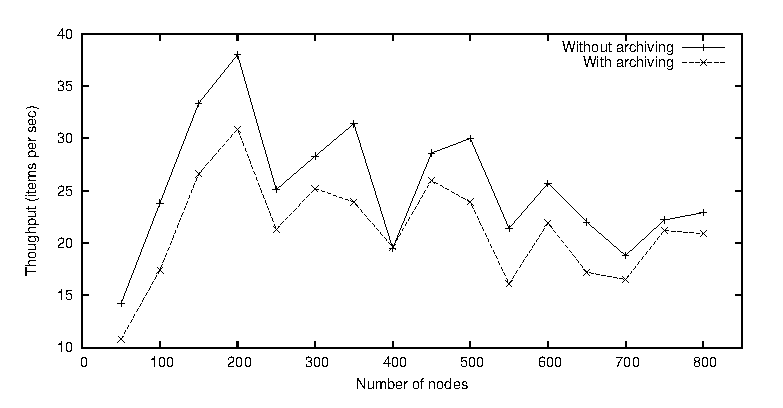
\epsfig{file=throughput.eps, width=\columnwidth}
\caption{Average throughput}
\end{center}
\end{figure}

\begin{figure}
\begin{center}
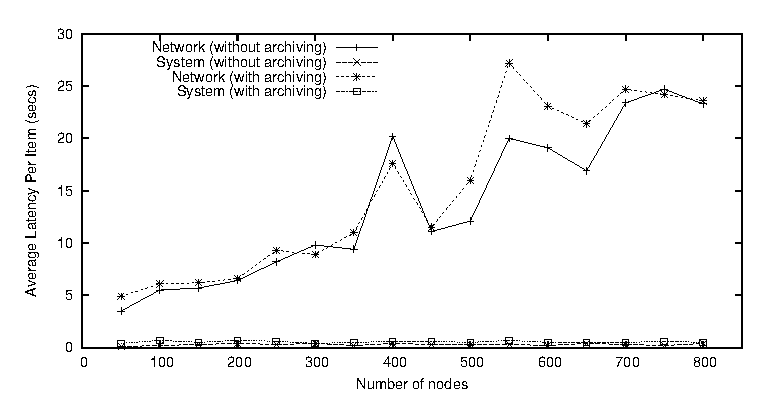
\epsfig{file=latency.eps, width=\columnwidth}
\caption{Average latencies per node}
\end{center}
\end{figure}


\begin{table*}
\begin{center}
\begin{tabular}{|l|r|r|r|r|r|r|r|r|r|r|r|r|}\hline
Num of nodes&	50&	100&	150&	200&	250&	300&	350&	400&	450&	500&	550&	600 \\ \hline\hline
Net latency per node (secs)&	9&	4&	4&	4&	8.6&	5.3&	19.1&	19.5&	14.4&	7.8&	12&	13.3 \\ \hline
Sys latency per node (secs)&	0&	0&	0&	0.3&	0.2&	0.4&	0.3&	0.1&	0.3&	0.4&	0.2&	0.7 \\ \hline
%Total Latency (secs)&	9&	4.04&	4&	4.3&	8.8&	5.8&	19.4&	19.6&	14.7&	8.2&	12.3&	14 \\ \hline
Total fetch time (secs)&	9&	5&	4&	5&	23&	9&	22&	23&	26&	14&	27&	28 \\ \hline	
Throughput (items/sec)&	5.6&	20&	37.5&	40&	10.9&	33.3&	15.9&	17.4&	17.3&	35.7&	20.4&	21.4 \\ \hline
\end{tabular}
\end{center}
\caption{Performance of Comon with no archiving}
\end{table*}


\begin{table*}
\begin{center}
\begin{tabular}{|l|r|r|r|r|r|r|r|r|r|r|r|r|}\hline
Num of nodes&	50&	100&	150&	200&	250&	300&	350&	400&	450&	500&	550&	600 \\ \hline\hline
Net latency per node (secs)&	16&	4&	4&	4&	18.9&	6&	20.6&	22&	8.4&	13&	21.8&	21.3 \\ \hline
Sys latency per node (secs)&	0.8&	1.28&	1.4&	1.8&	1.9&	1.5&	1.6&	1.3&	1.9&	1.7&	1.7&	2.2 \\ \hline
%Total Latency (secs)&	16.8&	5.28&	5.4&	5.8&	20.8&	7.5&	22.2&	23.3&	10.3&	14.7&	23.56&	23.5 \\ \hline
Total fetch time (secs)&	17&	6&	7&	7&	27&	12&	27&	30&	19&	33&	43&	43 \\ \hline
Throughput (items/sec)&	2.9&	16.7&	21.4&	28.6&	9.3&	25&	13&	13.3&	23.7&	15.2&	12.8&	14 \\ \hline
\end{tabular}
\end{center}
\caption{Performance of Comon with archiving}
\end{table*}

\section{SWAT: A Case Study}
\label{sec:swat}

\section{Related Work}\label{sec:related}


The explosive growth of the internet has made monitoring and managing
data systems distributed across wide-area networks increasingly
important.  The possibility of partial failure and the need to
synchronize makes such code tedious and difficult to write correctly,
particularly for data experts whose skills are in domains other than
networking. In this paper, we describe the \padsd{} system, which
allows users to declaratively specify their data systems and then
generate a wide-variety of tools for manipulating the data: from
stand-alone tools, to simple libraries for writing their own analyses,
to generic libraries for building new generic tools.  We precisely
specify the meaning of our language via a sound denotational
semantics and show via experimentation that the system has
acceptable performance overheads.
 
\bibliographystyle{plain} 
\balance  
\bibliography{main}

\end{document}
